\documentclass[english]{article}
\usepackage[T1]{fontenc}
\usepackage[utf8]{inputenc}
\usepackage[italian]{babel}
\usepackage{graphicx}
\usepackage{subcaption}
\usepackage{caption}
\usepackage{gensymb}
\usepackage{amsmath,bm}
\usepackage{siunitx}
\usepackage{float}
\usepackage{hyperref}
\captionsetup{tableposition=top,figureposition=bottom,font=footnotesize}
\renewcommand{\vec}{\mathbf}
\usepackage{upgreek}
\usepackage[a4paper, total={7in, 8in}]{geometry}
\begin{document}
\title{TITOLO:RELAZIONE DI DATA MINING}
\author{Daniele Maria Di Nosse, Angelo Lasala, Raffaele Paradiso}
\date{21/11/2020\newpage}

\maketitle
\tableofcontents{}

\newpage

\section{Clustering}
\subsection{DBSCAN}
Oltre l'algoritmo del KMeans per la ricerca di cluster ne esistono altri tra cui il DBSCAN (Density-based spatial clustering of applications with noise).
Il DBSCAN ricerca regioni localizzate con un'elevata densità di punti e le separa dalle regioni con una densità più bassa. Il problema principale dell'utilizzo di questo algoritmo è rappresentato dal "tuning" dei parametri che definiscono l'algoritmo, l'$eps$ che rappresenta la massima distanza tra due set di punti e $min$ $samples$ ovvero il numero di punti necessari (incluso il punto stesso) affinchè un set di punti possa essere considerato un core point.\\ 

StandardScaler removes the mean and scales the data to unit variance.\\
RobustScaler scale features using statistics that are robust to outliers. This Scaler removes the median and scales the data according to the quantile range (defaults to IQR: Interquartile Range). The IQR is the range between the 1st quartile (25th quantile) and the 3rd quartile (75th quantile). Centering and scaling happen independently on each feature by computing the relevant statistics on the samples in the training set. Median and interquartile range are then stored to be used on later data using the transform method. Typically this is done by removing the mean and scaling to unit variance. However, outliers can often influence the sample mean / variance in a negative way. In such cases, the median and the interquartile range often give better results.\\
MinMaxScaler rescales the data set such that all feature values are in the range [0, 1].
As StandardScaler, MinMaxScaler is very sensitive to the presence of outliers.\\
\begin{figure}[H]
\begin{minipage}[b]{0.45\textwidth}
\centering
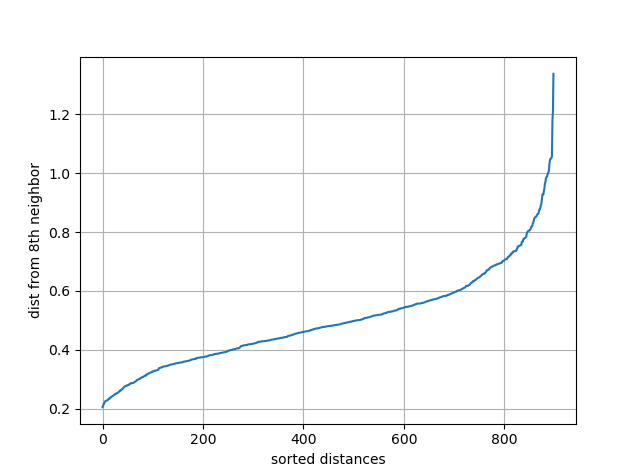
\includegraphics[width=\textwidth]{./Figure/Cluster/dbscan/1/Figure_1.png}
\caption{Didascalia 1.}
\label{etichetta1}
\end{minipage}
\hfill
\begin{minipage}[b]{0.45\textwidth}
\centering
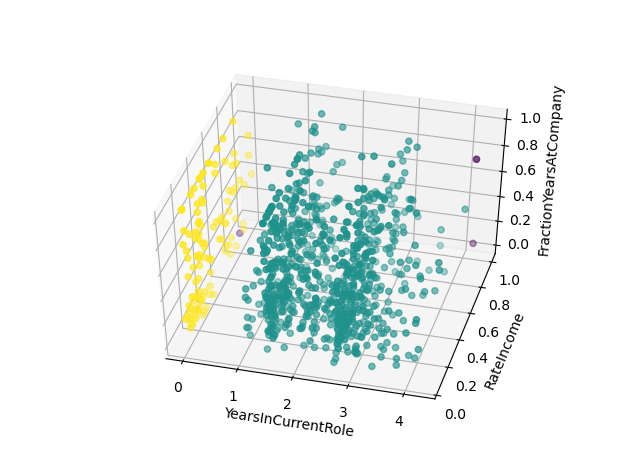
\includegraphics[width=\textwidth]{./Figure/Cluster/dbscan/1/Figure_24.png}
\caption{Didascalia 2.}
\label{etichetta2}
\end{minipage}
\end{figure}


\begin{figure}[H]
\begin{minipage}[b]{0.45\textwidth}
\centering
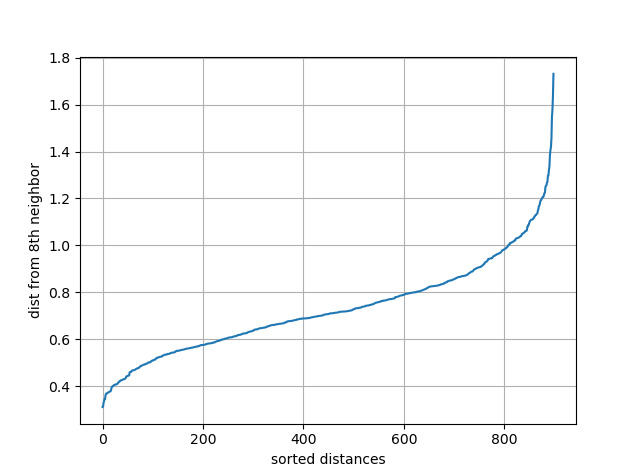
\includegraphics[width=\textwidth]{./Figure/Cluster/dbscan/2ok/Figure_1.png}
\caption{Didascalia 1.}
\label{etichetta1}
\centering
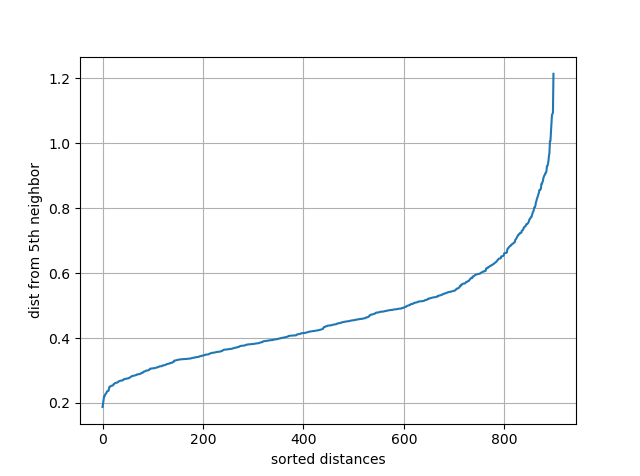
\includegraphics[width=\textwidth]{./Figure/Cluster/dbscan/4/Figure_1.png}
\caption{Didascalia 1.}
\label{etichetta1}
\centering
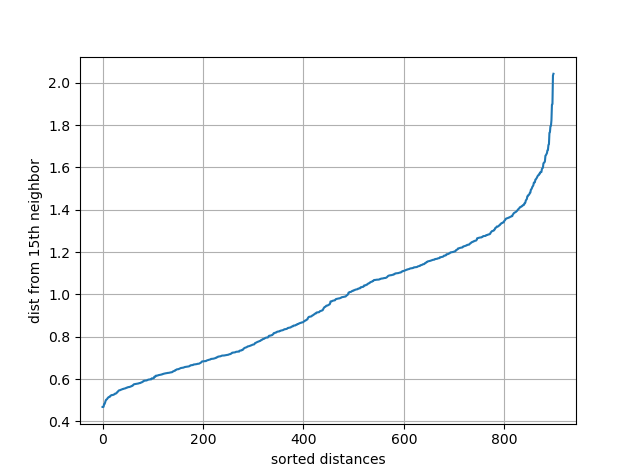
\includegraphics[width=\textwidth]{./Figure/Cluster/dbscan/5/Figure_1.png}
\caption{Didascalia 1.}
\label{etichetta1}
\end{minipage}
\hfill
\begin{minipage}[b]{0.45\textwidth}
\centering
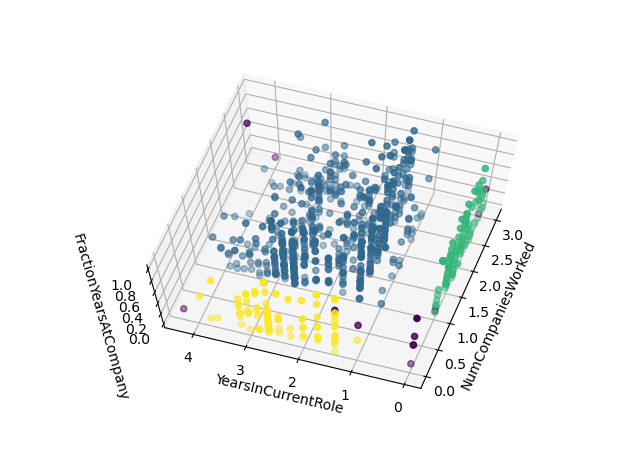
\includegraphics[width=\textwidth]{./Figure/Cluster/dbscan/3/Figure_24.png}
\caption{Didascalia 2.}
\label{etichetta2}
\centering
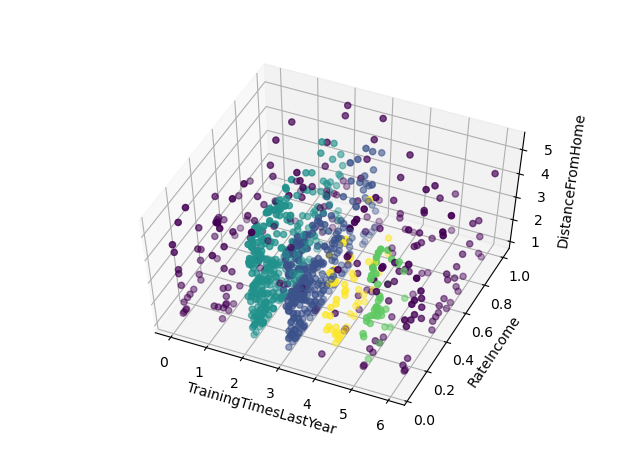
\includegraphics[width=\textwidth]{./Figure/Cluster/dbscan/5/Figure_5.png}
\caption{Didascalia 2.}
\label{etichetta2}
\centering
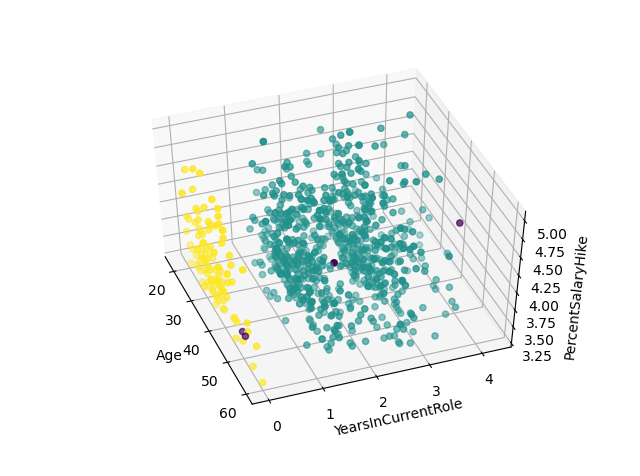
\includegraphics[width=\textwidth]{./Figure/Cluster/dbscan/4/Figure_21.png}
\caption{Didascalia 2.}
\label{etichetta2}
\end{minipage}
\end{figure}

\begin{figure}[H]
\begin{minipage}[b]{0.45\textwidth}
\centering
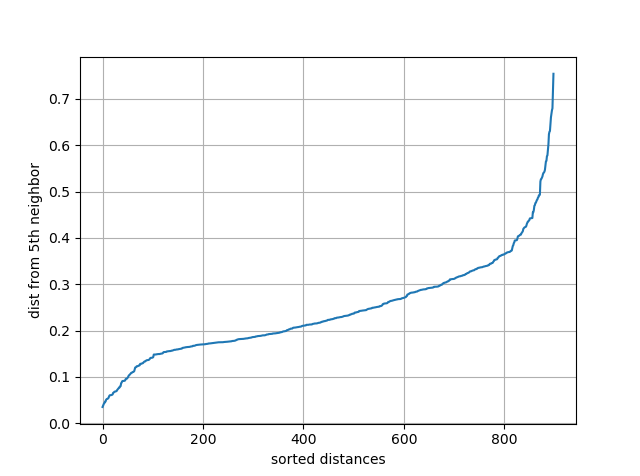
\includegraphics[width=\textwidth]{./Figure/Cluster/dbscan/6/elbow.png}
\caption{Didascalia 1.}
\label{etichetta1}
\end{minipage}
\hfill
\begin{minipage}[b]{0.45\textwidth}
\centering
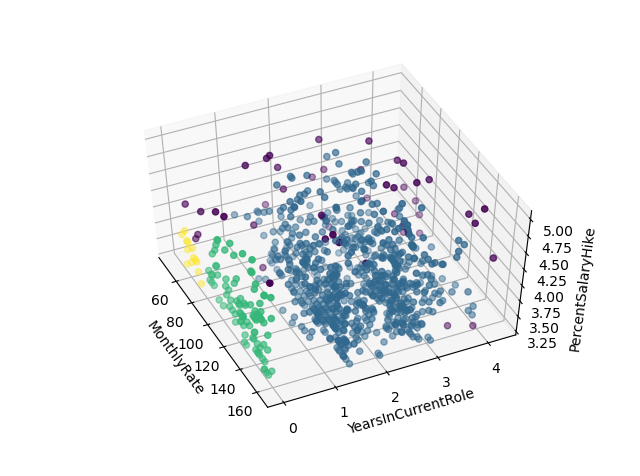
\includegraphics[width=\textwidth]{./Figure/Cluster/dbscan/6/Figure_6.png}
\caption{Didascalia 2.}
\label{etichetta2}
\end{minipage}
\end{figure}



%scaler = MinMaxScaler()
%X = scaler.fit_transform(df.values)
%dbscan = DBSCAN(eps=0.22, min_samples=5)
%dbscan.fit(X)
%
%labels_: Cluster labels for each point in the dataset. Noisy samples are given the label -1.
%
%Observing the size of each cluster
%
%Clustering Validation
%Silhouette
%
%%Knee Method to estimate the best eps
%
%dist = pdist(X, 'euclidean') #pair wise distance
%print (dist)
%dist = squareform(dist) #distance matrix given the vector dist
%print()
%print(dist)
%
%k = 5
%kth_distances = list()
%for d in dist:
%    index_kth_distance = np.argsort(d)[k]
%    kth_distances.append(d[index_kth_distance])
%plt.plot(range(0, len(kth_distances)), sorted(kth_distances))
%plt.ylabel('dist from %sth neighbor' % k, fontsize=18)
%plt.xlabel('sorted distances', fontsize=18)
%plt.tick_params(axis='both', which='major', labelsize=22)
%plt.show()

Advantages
DBSCAN does not require one to specify the number of clusters in the data a priori, as opposed to k-means.
DBSCAN can find arbitrarily-shaped clusters.
DBSCAN requires just two parameters and is mostly insensitive to the ordering of the points in the database. 
Disadvantages
DBSCAN is not entirely deterministic: border points that are reachable from more than one cluster can be part of either cluster, depending on the order the data are processed.
The quality of DBSCAN depends on the distance measure used in the function regionQuery$(P,eps)$. 
The most common distance metric used is Euclidean distance. 
Especially for high-dimensional data, this metric can be rendered almost useless due to the so-called "Curse of dimensionality", making it difficult to find an appropriate value for $eps$. 
This effect, however, is also present in any other algorithm based on Euclidean distance. 
DBSCAN cannot cluster data sets well with large differences in densities, since the $minPts-eps$ combination cannot then be chosen appropriately for all clusters.
If the data and scale are not well understood, choosing a meaningful distance threshold eps can be difficult.\\
\newpage

\section{Conclusioni}
\end{document}
